Where we previously assumed the existence of an ideal payment procedure, we now
describe our construction for the moneTor payment scheme. We first summarize the
algorithmic design of our payment protocols and proceed to describe integration
details with the Tor networking layer and codebase.

\subsection{Security Model}

The security model must account for both privacy and payment security. The
privacy threat model is derived from the local active adversary paradigm
ubiquitously found in Tor research~\cite{dingledine2004tor}. Informally, we
claim the following anonymity guarantees relative to unmodified Tor:

\begin{enumerate}
\item No additional party needed to operate the moneTor system (i.e. ledgers
  and intermediaries) will know any more about a given user than would be known
  by an additional middle relay.
\item In typical usage, circuits do not leak any more information other than the
  single bit needed to differentiate premium and nonpremium users.
\end{enumerate}

Our threat model for payment security is similar to those found in prior works
in blockchain micropayment channels~\cite{poon2016bitcoin}. In such models, the
user is protected from malicious intermediaries by the ability to prove
misbehavior to a global ledger. The security guarantees on the ledger will be
subject to the guarantees made by the cryptocurrency
interface~\cite{back2014enabling, poon2017plasma}. This is in direct contrast to
prior Chaumian e-cash proposals that employ the \emph{honest but curious} model
for the central bank. In moneTor, users funds are never controlled by external
authorities. Indeed, this is the basis for differenting the terminology between
prior \emph{central banks} and the moneTor \emph{Ledger}.

\subsection{Payment Protocols}

In this section we specify formal protocols that comprise the payment
scheme. All protocols are either two or three party interactions between a
subset of the following roles: $C$ (client), $R$ (relay), $E$ (end user: either
a client or relay), $I$ (intermediary), and $L$ (ledger). At this level, we
assume that one client is paying one relay through a single channel and that
network-layer anonymity will be appropriately handled at the Tor protocol level.

\textbf{Bolt} The full moneTor payment scheme is a superset of Bolt three-party bidirectional
micropayment channels and, as such, we adopt its nomenclature where possible but
adapt it to our concepts of ledgers, clients, relays, etc. The following is brief
outline of the prerequisite micropayment channel procedures defined in Bolt. We
refer the reader to the original paper for more detailed
specifications~\cite{green2017bolt}.

\begin{itemize}
\item $KeyGen$: Any party generates a cryptographic keypair
\item $Init_E$: $E$ initializes her half of a micropayment channel by escrowing
  initial funds on $L$
\item $Init_I$: $I$ initializes his half of a micropayment channel by
  escrowing intial funds on $L$
\item $Establish$: $E$ and $I$ interact to establish a new, functional
  micropayment channel
\item $Pay$: $E_1$ interacts with $I$ and $E_2$ to send a single micropayment to $E_2$
\item $Refund$: $E$ closes a micropayment channel on $L$ and makes a claim on
  the escrowed balance.
\item $Refute$: $I$ closes a micropayment channel on $L$ and makes a claim on
  the escrowed balance.
\item $Resolve$: $L$ determines the final balance of funds awared to
  each party.
\end{itemize}

While anonymous micropayment channels present a tremendous advance for many
applications, the relatively heavy cryptography ($37-100 ms$) and communication
(7 message legs) is a prohibitive expense for Tor relay payment. In addition to
concerns regarding global network overhead, it is also desirable to keep the
barrior threshold low for small perspective relay operators. We therefore
introduce a new payment layer that enables the first practically efficient
payments for Tor routing.

\textbf{moneTor} The moneTor construction makes use of the existing anonoymous
micropayment structure to facilitate \emph{locally transparent nanopayments}. In
this scheme, \emph{nanopayment channels} are established in place of a single
micropayment operation. These lightweight channels allow the client to send a
$n$ number of undirectional nanopayments to the relay. Each payment represents a
fixed value $\delta$, established at the start of the channel. The payments
themselves are \emph{locally transparent} in the sense that each nanopayment in
the same channel is trivially linked to each other. However, the nanopayment
channels themselves are anonymous with respect to other nanopayment channels and
micropayment operations.

Generic parties $C$ and $R$ can construct a nanopayment channel once both have
completed $Establish$ with a commone intermediary $I$. We define the following
set of protocols needed to manage nanopayments.

\begin{itemize}
\item $Nano$-$Setup$: $C$ and $I$ interact to prepare a nanopayment channel on top
  of their existing micropayment channel.
\item $Nano$-$Establish$: $C$ sends her nanopayment channel information to $R$,
  who establishes it with $I$ on top of their existing micropayment channel.
\item $Nano$-$Pay$: $C$ sends a single nanopayment channel to $R$. This is
  repeatable for up to $n$ operations.
\item $Nano$-$Close_R$: $R$ closes his nanopayment channel with $I$.
\item $Nano$-$Close_C$: $C$ closes her nanopayment channel with $I$. Note that
  this must happen after $Nano$-$Close_R$.
\end{itemize}

We also specify the following modified channel conflict resolution procedures to
ensure secure closure properties for the nanopayment scheme.

\begin{itemize}
\item $Nano$-$Refund$: $E$ closes channel on $L$.
\item $Nano$-$Refute$: $I$ closes channel on $L$.
\item $Nano$-$Resolve$: $L$ makes final determination on both micropayment and
  outstanding nanopayment balances.
\end{itemize}

The core of our nanopayment scheme is inspired by the classic \emph{Payword}
two-party micropayment scheme in which payments are encoded by successively
revealed preimages in a precomputed hash chain~\cite{rivest1996payword}. Hash
chains are perhaps the most efficient known method for representing payments. In
contrast to the expensive zero-knowledge proofs and signatures involved in
anonymous micropayments, hash chain payments can be computed one the order of
millions of hashes per second and conferred with a single 256 bit message, or
one Tor cell.

The challenge in this construction is to securely integrate the hash chain
concept into an existing three-party anonymous micropayment channel setup such
that all parties maintain secure cryptographic ownership of their funds at all
steps. At the same time, we must ensure that no deanonymizing information is
leaked outside of the nanopayment channel context. We proceed to present a
concrete scheme which incurrs an overhead penalty of approximately two
micropayment operations per nanopayment channel, one at the beginning and one at
the end of the channel lifecycle.

\subsection{Nanopayment Protocols}
In this section, we provide a summarized intuition for the basic steps in the
payment protocol. A more formal algorithmic treatment of the steps are provided
in Appendix~\ref{sec:algorithms}.

\textbf{Nano-Setup} At the start of this protocol, $C$ has access to a
micropayment wallet $w$ that enables her to operate her micropayment channel
with $I$ as well as a refund token $rt$ that entitles her to claim her current
funds on $L$ should $I$ misbehave or go offline. To construct a nanopayment
channel, $C$ first generates an array of values $hc$ of length $n$ where
$hc_i = H(hc_{i+1})$ and $hc_n$ is a random number. The root of the hash chain
$hc_0$ is used to create a globally unique nanopayment token $nT$ that encodes
the public parameters of the channel including the length $n$ and the
per-payment value $\delta$. $C$ sends $I$ a commitment to a fresh nanopayment
channel parametrized by $nT$ along with a zero-knowledge proof of the following
statements:

\begin{enumerate}
\item The nanopayment wallet $nw$ is well-formed from $w$
\item $C$ has ownership of a micropayment channel containing at least $n *
  \delta$ funds.
\end{enumerate}

$I$ verifies these messages and blindly supplies $C$ with a new refund token
$nrt$ that entitles $C$ to cash out the full balance of the micropayment channel
along with any nanopayments to $L$. $C$, now protected against misbehavior by
$I$, agrees to send a revocation token $\sigma_w$, which revokes her right to
use $w$ or $rt$. $I$, now protected against double spending by $C$, can safely
inform $C$ that the nanopayment channel has been set up successfully.

\textbf{Nano-Establish} At this point, $C$ sends $R$ the same $nT$ token used to
setup the channel with $I$. $R$ uses the token to initiate her end of the
nanopayment channel with $I$ by executing essentially the same procedure that
$C$ used in $Nano$-$Setup$. The nanopayment channel is now fully established and
ready to be used. A key observation is that both ends of the channel ($C$-$I$
and $R$-$I$) are rooted at the same hash chain root $hc_0$. As a result, the
scheme satisfies the correct-by-construction property of \emph{atomicity}
whereby both legs of the protocol are finalized at the same time.

\textbf{Nano-Pay} To make the next $i^{th}$ payment, $C$ simply sends the next
hash preimage $hc_i$ to $R$. Knowledge of this preimage $hc_i$ is sufficient for
$R$ to prove posession of a nanopayment. At any given time, $R$ can broadcast
the tuple ($nrt$, $hc_i$) to $L$ to prove ownership of the correct balance of
funds. Notice that this action simultaneously reveals $hc_i$ to $I$, who can
then claim an equivalent value of funds from $C$.

\textbf{Nano-Close} After some number of payments $k < n$ has transpired, $C$ and $R$ will both wish
to close their nanopayment channels through $I$. In this process, the $R$-$I$ leg
must be closed before the $C$-$I$ leg. This is due to the unidirectional nature
of nanopayment channels. Since payments are flowing form $C$ to $R$, $I$ must
first determine its debt to $R$ in order to know how much it can claim from $C$.

$R$ first sends to $I$ a commitment to a new micropayment wallet $w'$ and a
zero-knowledge proof of the following statements:

\begin{enumerate}
\item $w'$ is well-formed from $w$
\item The balance of $w'$ is equal to the sum of the previous wallet $w$ and
  $\delta * k$
\end{enumerate}

Once verified, $I$ issues a refund token $rt'$ on the new funds. $R$ agrees to
invalidate the nanopayment channel by issuing a revocation token $\sigma_{nw}$
to $I$. $I$ and $R$ proceed to create a blind signature on $w'$ thus validating
the wallet for future use.

Once $I$ has closed his nanopayment channel leg with $R$, $I$ and $C$ are free
to complete the exact same close protocol. All parties are now reverted to the
original state they occupied prior to $Nano$-$Setup$ save for a securely updated
balance.

\subsection{Payment Implementation}

We implement the abstract payment protocols as a series of well-isolated
\emph{payment modules}, one for each of $C$, $R$, $I$, and $L$. The payment
module interacts with the rest of the Tor codebase through a network-layer
\emph{controller} which defines emphemeral descriptors that the module uses to
communicate with other payment modules across the network. The controller
exposes $send$ and $recv$ functionality to the payment module, which in turn
accepts $pay$, $close$, and $cashout$ requests. We anticipate that this API is
general enough to isolate many future changes which may occur in either
component.

The concrete implementation also warrants some additional remarks. Up to this
point, we have described payments that happen between a single client and a
single relay. In reality, it is typical for each client to manage a handful of
concurrently active circuits,\footnote{For instance, the popular Tor Browser
  user applicaiton dedicates a separate circuit for each tab~[can we cite?]}
each of which requires three streams of payment to the guard, middle, and exit
relays. An interesting area of future work involves optimizing payment channels
to balance both the computational resources as well as escrowed financial
capital that active channels consume. As a separate remark, we only define
protocols for the most general case in which we require maximal payment
anonymity. However, a fundamental feature of the Tor network is the fact the
transparent relationship between a client and its guard relay is persistent
across the timescale of months. We exploit this setup to allow for extremely
efficient direct payment channels between the client and guard, considerably
reducing the network overhead costs.

\subsection{Network Protocol and Implementation}
%talk about leaky-pipe topology
%needs an overview of the protocol extension and some nicelydone image
%some theoretical discussion about how to properly anonymize R->I, C->I, R/C->L connections using Tor circuits.
%memory cost/cpu cost discussion

\subsubsection{Extending the Tor protocol}
We extend the Tor routing protocol described in Tor's specifications~\cite{torspec} and we exploit Tor's leaky-pipe circuit topology to exchange payment information with each hop of the circuit (i.e., the Tor protocol allows a client to direct traffic partway down the circuit). We introduce two new control cell types: one link-level cell and one relay-level cell. The link-level cell is used to exchange information related to the payment protocol between the Tor client and its guard relay. This cell is not onion-encrypted (but the TLS layer still protect it) and is not used for any other purpose. The relay-level cell is used to exchange payment information with the middle relay and the exit relay: 2 onion-encryptions makes the cell exiting the circuit at the middle relay. 3 onion-encryptions makes the cell exiting the circuit at the usual exit relay for data streams. This subtype of relay cell is indistinguishable from a normal relay cell and carries a header related to the payment system, followed by a payload of payment data. Figure~\ref{fig:relay_command_mt_structure} shows the internal structure of the cell.

\begin{figure}[h]
	\centering
	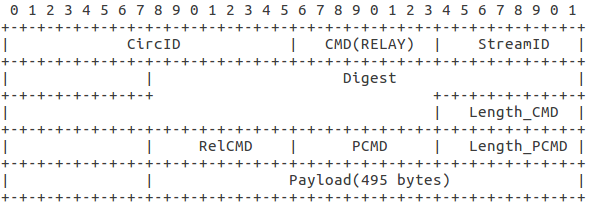
\includegraphics[scale=0.38]{images/payment_cell_header.png}
	\label{fig:relay_command_mt_structure}
	\caption{Relay level payment cell structure}
\end{figure}

All the bytes starting from StreamID (included) are onion-encrypted. RelCMD is set to RELAY\_COMMAND\_DATA, PCMD is the payment command which is different for each step of the payment protocol. If some message overflow the payload available length (495 bytes), we queue multiple cells of the same PCMD and buffer them on the receiver side to unpack the whole message.

\subsubsection{Payment Anonymity}

\td{TODO: describes the communiction circuits needed to make anonymous payments
  without stupidly revealing identity via network addresses}

\subsubsection{Scalability Design of the moneTor Scheme}

\td{TODO: describe scalability of intermediary system and any networking
  bottlenecks that might arise such as port limits, etc.}